\documentclass{article}
\usepackage{graphicx}
\usepackage{float}

\title{Labwork 3: Hello, CUDA!}
\author{Vu Ha Vy -- 2540112}
\date{\today}

\begin{document}

\maketitle

\section{CPU vs. GPU Performance}

In this experiment, the input image was processed on both CPU and GPU. 

\begin{figure}[H]
\centering
\begin{minipage}{0.45\textwidth}
  \centering
  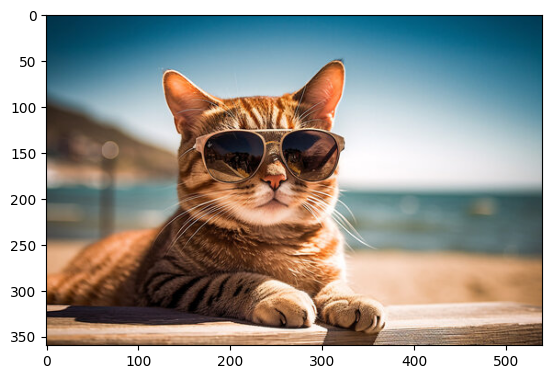
\includegraphics[width=\textwidth]{picture/input.png}
  \caption{Input Image}
\end{minipage}
\hfill
\begin{minipage}{0.45\textwidth}
  \centering
  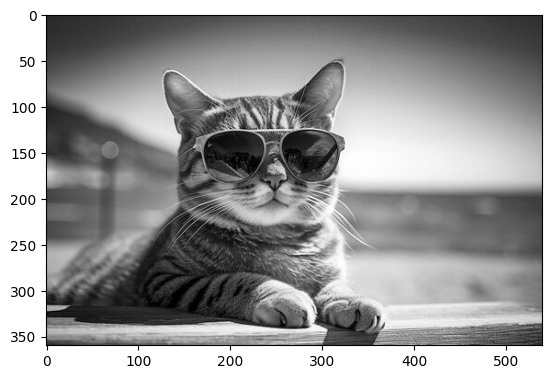
\includegraphics[width=\textwidth]{picture/output.png}
  \caption{Output Image}
\end{minipage}
\end{figure}

\subsection*{CPU Implementation:}
The CPU processes pixels sequentially through a loop, calculating the average RGB value to produce a grayscale pixel and assigning it to all three color channels. It then calls this function on the flattened image and reshapes the output array back into the original 2D image dimensions. \\

\noindent\textit{for i in range(len(src)):} \\
\textit{\hspace*{1.5em}g = np.uint8((int(src[i,0]) + int(src[i,1]) + int(src[i,2])) / 3)} \\
\textit{\hspace*{1.5em}dst[i,0] = dst[i,1] = dst[i,2] = g} 
\smallskip
\textit{cpuDst = grayscale\_cpu(flatImg)} \\
\smallskip
\textit{cpuImg = cpuDst.reshape(height, width, 3)}

\subsection*{GPU Implementation:}

The GPU implementation processes pixels concurrently using parallel CUDA threads, where each thread identifies its target element using a global index derived from \texttt{cuda.threadIdx.x}, \texttt{cuda.blockIdx.x}, and \texttt{cuda.blockDim.x}. Data is transferred from host memory to device memory using \texttt{cuda.to\_device()} before launching the \texttt{@cuda.jit} kernel across the grid. Once parallel execution completes on the GPU, the result is transferred back to system memory via \texttt{copy\_to\_host()} and reshaped into the final image dimensions. \\

\noindent\textit{tidx = cuda.threadIdx.x + cuda.blockIdx.x * cuda.blockDim.x} \\
\textit{g = np.uint8((src[tidx, 0] + src[tidx, 1] + src[tidx, 2]) / 3)} \\
\textit{dst[tidx, 0] = dst[tidx, 1] = dst[tidx, 2] = g} \\
\smallskip
\textit{devSrc = cuda.to\_device(flatImg)} \\
\textit{devDst = cuda.device\_array(flatImg.shape, np.uint8)} \\
\textit{grayscale[gridSize, blockSize](devSrc, devDst)} \\
\textit{hostDst = devDst.copy\_to\_host()} \\
\smallskip
\textit{gpuImg = hostDst.reshape(height, width, 3)}

\subsection*{Running time}

\begin{table}[H]
\centering
\renewcommand{\arraystretch}{1.5}
\begin{tabular}{|l|c|}
\hline
\textbf{Implementation} & \textbf{Running Time (s)} \\ \hline
CPU & 0.3203566074371338 \\ \hline
GPU & 0.09885144233703613 \\ \hline
\end{tabular}
\caption{Running Time Comparison}
\end{table}

\noindent \textbf{Conclusion:} The GPU implementation had a speedup of approximately 3.24x compared to the CPU implementation, reducing the processing time from 0.320 seconds to 0.099 seconds.

\section{Impact of CUDA Block Size}

\begin{table}[H]
\centering
\renewcommand{\arraystretch}{1.5}
\begin{tabular}{|c|c|}
\hline
\textbf{Block size} & \textbf{Running Time (s)} \\ \hline
32 & 0.004130840301513672 \\ \hline
64 & 0.0010914802551269531 \\ \hline
128 & 0.003341197967529297 \\ \hline
256 & 0.0018801689147949219 \\ \hline
512 & 0.0017004013061523438 \\ \hline
\end{tabular}
\caption{Execution Time for Different Block Sizes}
\end{table}

\begin{figure}[H]
\centering
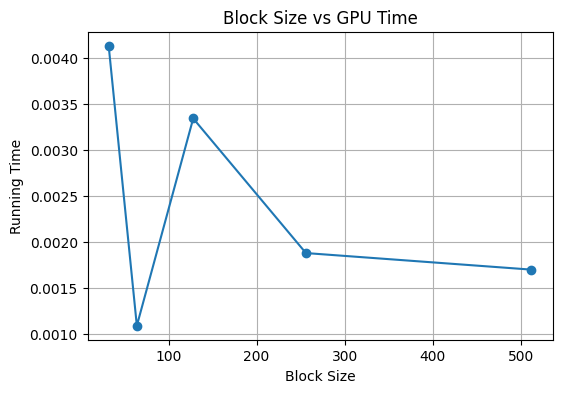
\includegraphics[width=1\textwidth]{picture/compare.png}
\caption{Running Time Across Different CUDA Block Sizes}
\end{figure}

\noindent \textbf{Pattern Analysis:} \\
The execution time decreases significantly from a block size of 32 to 64, reaching the fastest performance at 64 (approx. 0.00109 seconds). However, increasing the block size to 128 caused a slowdown, and then the performance leveled off around 0.0017s - 0.0018s for 256 and 512. This shows that increasing block size does not strictly increase the performance. It also relies on balancing thread occupancy and hardware resource allocation per streaming multiprocessor.

\end{document}